% Horizon penetrating coordinates (vs. Schwarzschild coordinates)
% for a black hole spacetime, with excision
% Author: Jonah Miller
\documentclass[tikz,border=0pt]{standalone}
\usepackage{tikz}
\usepackage{pgf}
\usetikzlibrary{arrows}
\usetikzlibrary{arrows.meta}
\usetikzlibrary{automata}
\usetikzlibrary{positioning}
\usetikzlibrary{decorations.markings}
\usepackage{pgfplots}
\usepackage{xcolor}

%\tikzset{>={Latex[length=3mm]}}

\begin{document}
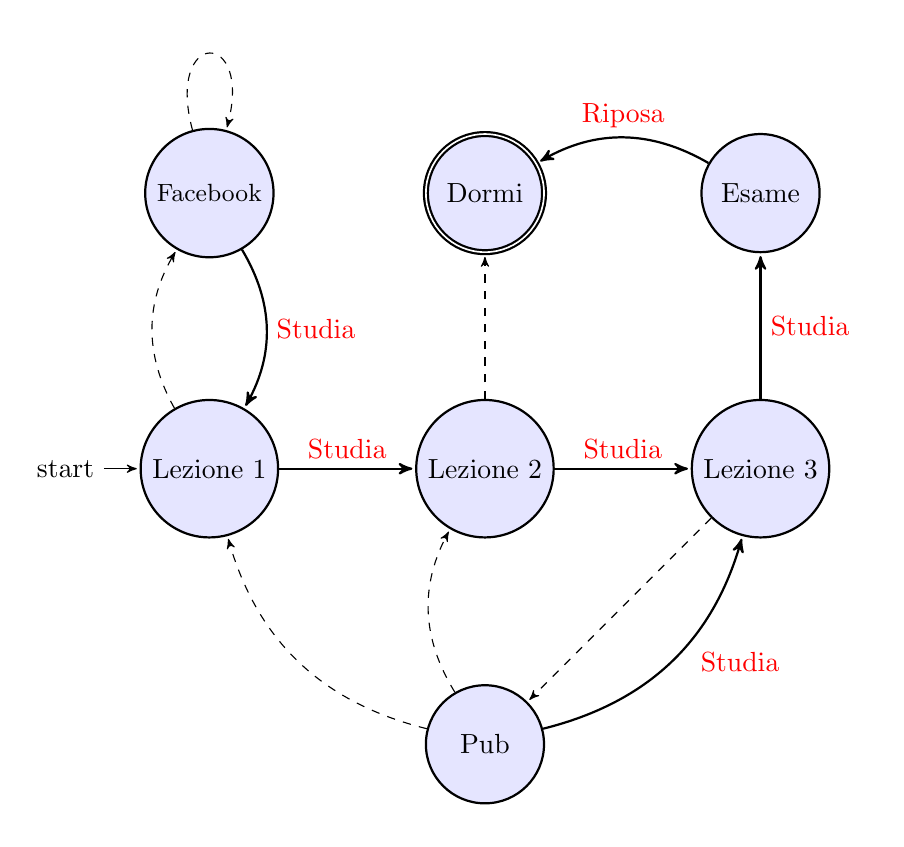
\begin{tikzpicture}[->, >=stealth', shorten >= 1pt, node distance=3.5cm]
\tikzstyle{every state} = [draw=black, text=black, minimum size=1.5cm, thick, fill=blue!10]

\node[state] (A) {\small Facebook\normalsize};
\node[state, initial] (B)[below of=A] {Lezione 1};
\node[state] (C)[right of=B] {Lezione 2};
\node[state] (D)[right of=C] {Lezione 3};
\node[state] (E)[above of=D] {Esame};
\node[state] (F)[below of=C] {Pub};
\node[state, accepting] (G)[above of=C] {Dormi};

\draw (A) node[text=red, xshift=1cm, yshift=-0.7cm)] {\hphantom{r=-1}};
\draw (B) node[text=red, xshift=1cm, yshift=-0.7cm)] {\hphantom{r=-2}};
\draw (C) node[text=red, xshift=1cm, yshift=-0.7cm)] {\hphantom{r=-2}};
\draw (D) node[text=red, xshift=1cm, yshift=-0.7cm)] {\hphantom{r=-2}};
\draw (E) node[text=red, xshift=0cm, yshift=1cm)] {\hphantom{r=+10}};
\draw (F) node[text=red, xshift=1cm, yshift=-0.7cm)] {\vphantom{r=+1}};
\draw (G) node[text=red, xshift=1cm, yshift=-0.7cm)] {\hphantom{r=0}};


\path (A) edge[bend left,thick] node[right, text=red]{Studia} (B)
			edge[loop above, dashed] node[above]{}	(A)
	(B) edge[bend left, dashed] node[left]{\hphantom{0.5}} (A)
		edge[thick] node[above, text=red]{Studia} (C)
	(C) edge[dashed] node[left]{} (G)
		edge[thick] node[above, text=red]{Studia} (D)	
	(D) edge[dashed] node[below,right]{} (F)
		edge[thick] node[right,text=red]{Studia} (E)
	(E) edge[bend right,thick] node[above=0pt,text=red]{Riposa} (G)
	(F) edge[bend left,dashed] node[left]{} (B)
		edge[bend left,dashed] node[left]{} (C)
		edge[bend right,thick] node[right=7pt,text=red]{Studia} (D) 
	;

\end{tikzpicture}
\end{document}